\section{Item}\label{sec:recipe}
As mentioned in \cref{sec:runningexample} a group of identical items to be produced by a factory are described by a recipe. This is a linear sequence of work, we need to perform on an item to complete it. Yet, we realize that a recipe need not be described as linear. In fact, in some cases we do not care about the order of work. 

Let us look back to the linear recipe, describing how a doll should be produced on \cref{fig:running-example}. It states that the doll must have arms, legs and head attached in the given order. Yet, we may not care for the order in which we attach limbs. Therefore we model a recipe not as a sequence, but an acyclic dependency graph as seen in \cref{fig:dependency-graph}. If node $A$ has an edge going to another node $B$, $A$ is said to depend on $B$. In our case, it means that the work, which $B$ represents, should be accomplished before $A$. 

The doll recipe now states that after a doll base has been loaded onto the factory, we may attatch arms, legs and head in any order. Yet we may not paint the doll before all limbs have been attached, and we can not gift wrap the doll before it has been painted. This lets us set up more complex recipes that we may produce items according to. 

Since the graph is acyclic, we may not model items, where their recipes require the same work performed twice. This may happen in the real world, yet we look past it, as many types of recipes pass this restriction. As an example, while the inspected CP-learning factory configuration has physical cycles in its layout, but no item produced on it is made according to a recipe that requires the same work performed twice.  

\begin{figure}[H]
\centering
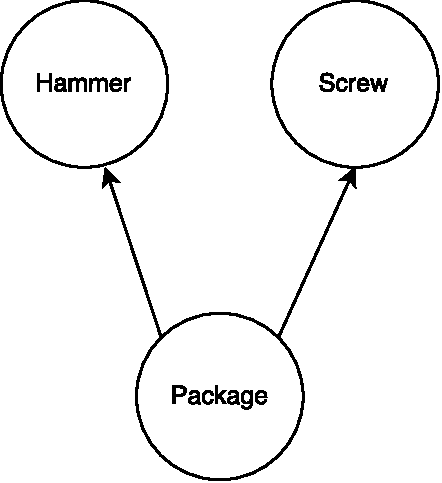
\includegraphics[width=0.3\textwidth]{dependencygraph.pdf}
\caption{Acyclic dependency graph describing order of actions}
\label{fig:dependency-graph}
\end{figure}

Neither do we model items, which distribute their production. This means that an item may have different parts located on different modules at the same time. Going back to the doll, this would allow us to paint the arms, legs head and base of the doll before putting it all together. To simplify our model we look past this. Thus, an item can only be located on a single module at one point in time. At the same time, no recipe may require that an item begins production from more than one specific module. At the local CP-learning factory we see no distributed production of any item. Therefore we can still describe production of real life items by modeling a recipe with an acyclic dependency graph.

In UPPAAL we may simulate the process of production by composing several smaller processes to run in parallel. Each process is instantiated through the use of a template. Templates are similar to classes in object oriented programming. Yet they consist not only of local variables and functions, but also a graphically designed timed automata. When a template is instantiated it evaluates to a process defined by initial parameters as well as the initial location of the timed automata. The restrictions set up by local variables, functions and timed automata  describe how this process may transform into other processes.   

To simulate production on a configuration, we must have several processes running in parallel. Some of these processes are of different types, which means that we need to set up different templates. In the following subsections we describe, how we model items in UPPAAL with the \textit{Item} template, so that we may simulate their production. In addition, we describe how we enforce the order in which items begin production using the \textit{ItemQueue} template.

\subsection{Item Template}\label{subs:recipe}
We could choose to implement a new template for each recipe, using it do instantiate items, which are described by that recipe. This would require no local functions in the template, as we could just translate the acyclic dependency graph, which describes the given recipe, to a timed automata. However, as revealed i\cref{ch:configuration_optimization}, we want to  instantiate our configurations in UPPAAL through python. To do this we alter the XML file, which describes our templates as well as details on the configuration to be run. Because of the structure of this file, it is easier to change local functions and variables of a template than the graphically designed timed automata. Therefore, we instead create a single template \textit{Item}, which is used to instantiate every item process. This template takes a recipe as an input parameter, to describe the work that the item requires.

A recipe is given as an array of nodes. For this we have developed a \textit{Node} struct as shown in \cref{code:Node}. A node knows what type of work it represents, the number of parents it has, its children's indexes in the node array and the number of children. Node $A$ is parent of node $B$, if $B$ depends on $A$, and the other way around for children. In addition to the recipe, we also give each item a unique id and the id of the module at which it begins production. 

\lstinputlisting[language=C, caption=Node struct, captionpos = b, label={code:Node}, float]{codeRelated/UPPAAL/node.txt}

The timed automata within the \textit{Item} template can be seen in \cref{fig:recipe}, initial location marked with a circle within a circle. From the initial location we may go to the \textit{InProgress} location, by placing the item onto its start module. In addition the transition requires a call to made to \textit{get\_upper\_nodes}. This instantiates the local \emph{current\_nodes} array to contain all nodes in the recipe, which do not depend on any other node. These describe the work, which we may initially be performed.  

After this, the item is moved along the factory. Each time it meets a module, where it wishes to have work done, it will handshake on its own private channel with the module to identify itself. Afterwards, it will synchronize with the module again on one of the allowed \emph{work} channels. A work channel can be synchronized on, if one of the nodes in the \emph{current\_nodes} array, represent the work corresponding to that work channel. This check is done by the \emph{is\_callable} function.

Before going back to the \emph{InProgress} location, a call to \emph{update\_current\_nodes} is made. The code of this function can be seen in \cref{code:updatecurrentnodes}. It will first collect all current nodes in the \emph{new\_nodes} array, except for \emph{called\_node}, as this is the node just worked on. It then runs over each of \emph{called\_node}'s children to decrement their \emph{number\_of\_parents} field by 1. If this field reaches 0, it means that the node no longer has any dependencies and can be worked on. Because of this, it is added to the \emph{new\_nodes} array. Once all children have been updated, the contents of \emph{new\_nodes} are used to update \emph{current\_nodes}. Thus we update the work, which we may perform according to the recipe.  

\lstinputlisting[language=C, caption={The update\_current\_nodes function local to the \textit{Item} template}, captionpos = b, label={code:updatecurrentnodes}, float]{codeRelated/UPPAAL/updatecurrentnodes.txt}

After the call to \emph{update\_current\_nodes} is finished, we call \emph{no\_more\_nodes}. This will set the local \emph{done} boolean to \emph{True}, if \emph{current\_nodes} nodes is empty. This means that the item can not be worked on any further. It has now been produced and may be removed from the factory.

\begin{figure}[H]
	\centering
	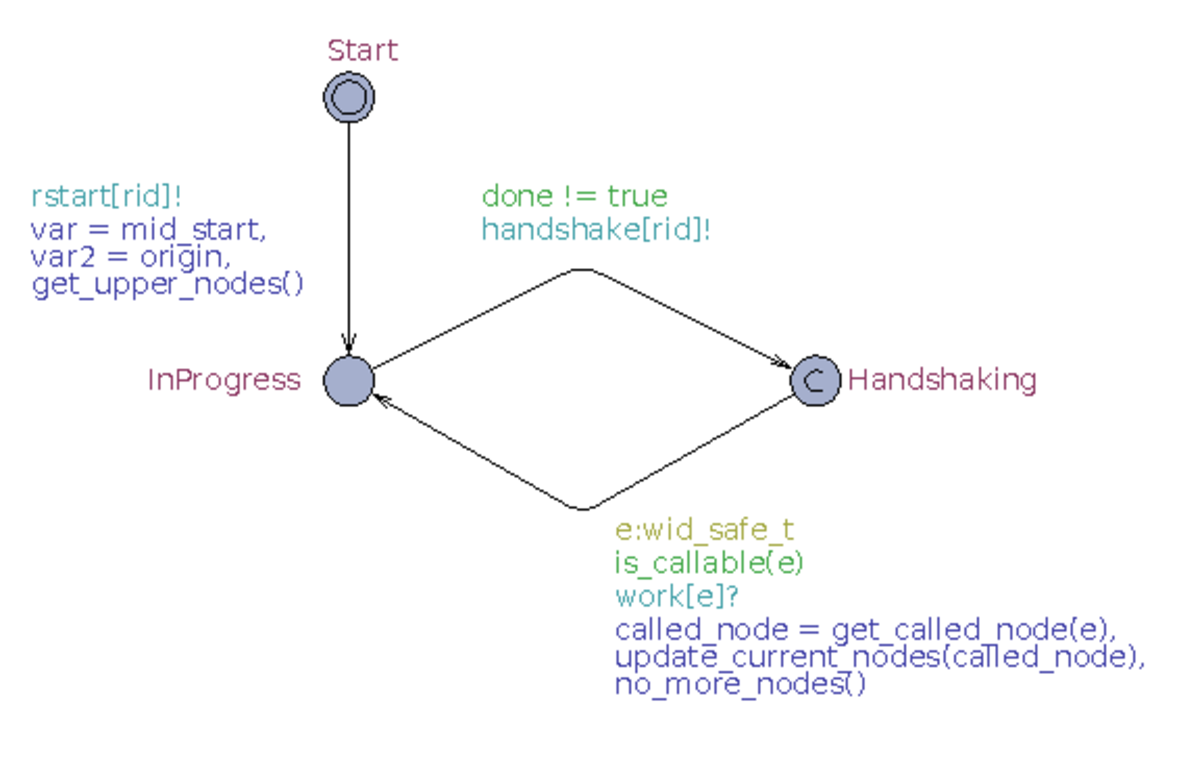
\includegraphics[width=\textwidth]{recipe.pdf}
	\caption{\textit{Item} template}
	\label{fig:recipe}
\end{figure}

\subsection{ItemQueue Template}\label{subs:recipequeue}

Having all item processes compete for a place on the factory at first, leads to a large state-space. This must be searched, when we ask UPPAAL to find the shortest timed trace. In order to get around this, we enforce a certain order, in which items may be placed onto the factory. This is done using a queuing system, which we implement using the \emph{ItemQueue} template as seen in \cref{fig:recipequeue}.

The template is instantiated with an array of item ids, indicating the order, in which we wish the items added. Once instantiated, the queue may begin dequeuing items, so that they may be placed onto the factory. This reduces the overall state space, as items are to begin in a specified order. 

\begin{figure}[H]
\centering
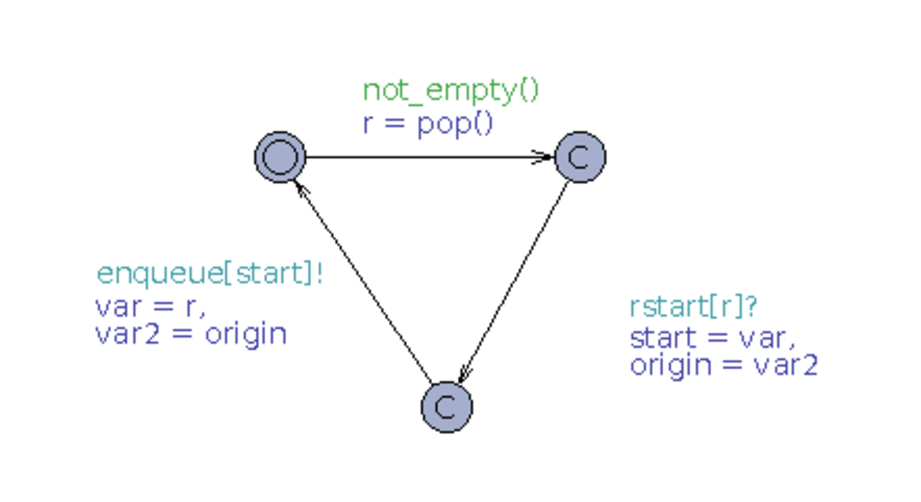
\includegraphics[width=\textwidth]{recipequeue.pdf}
\caption{\textit{ItemQueue} template}
\label{fig:recipequeue}
\end{figure}